%!TEX program = xelatex
\documentclass{beamer}
\usefonttheme[onlymath]{serif}
\usepackage{blindtext}
\usepackage{bm}
\usepackage{minted}
\usepackage{amsmath, amssymb}
\usepackage{tikzsymbols}
\usepackage[linesnumbered,ruled,vlined]{algorithm2e}
\newcommand\blfootnote[1]{%
  \begingroup
  \renewcommand\thefootnote{}\footnote{#1}%
  \addtocounter{footnote}{-1}%
  \endgroup
}

\usetheme{Execushares}

\title{Breaking Down Risk Parity Portfolios: A Practical Open Source Implementation}
\subtitle{a talk by}
\author{\textbf{Z\'e Vin\'icius}}
\date{Jan. 22nd, 2020}

\setcounter{showSlideNumbers}{1}

\begin{document}
	\setcounter{showProgressBar}{0}
	\setcounter{showSlideNumbers}{0}

	\frame{\titlepage}

        \begin{frame}
          \frametitle{whoami}
              \vspace{.5cm}
          \begin{itemize}
            \item made in Brazil
              \vspace{.25cm}
            \item electrical engineer by training, computer scientist by passion/experience
              \vspace{.25cm}
            \item guest researcher at NIST\footnote{National Institute of Standards and Technology, Washington DC, US}
              \vspace{.25cm}
            \item software developer for Google summer of code with OpenAstronomy
              \vspace{.25cm}
            \item software engineer intern NASA\footnote{National Aeronautics and Space Administration,
              Ames Research Center, Silicon Valley, US}
              \vspace{.25cm}
            \item \textbf{since Sept. 2019}: phd student at HKUST\footnote{The Hong Kong University of Science
              and Technology}
          \end{itemize}
        \end{frame}



	%\begin{frame}
	%	\frametitle{Contents}
	%	\begin{enumerate}
	%		\item Markowitz and Portfolio Optimization \\ \textcolor{ExecusharesGrey}{\footnotesize\hspace{1em} The reasoning and background behind this theme}
	%		\item   \\ \textcolor{ExecusharesGrey}{\footnotesize\hspace{1em} Just some Lorem Ipsum for filler}
	%		\item Conclusions \\ \textcolor{ExecusharesGrey}{\footnotesize\hspace{1em} Some closing thoughts}
	%	\end{enumerate}
	%\end{frame}

	\setcounter{showSlideNumbers}{0}
        \section{Portfolio Optimization}
	\setcounter{framenumber}{0}
	\setcounter{showProgressBar}{1}
	\setcounter{showSlideNumbers}{1}

  %\section{Markowitz and Portfolio Optimization}
  \begin{frame}
    \frametitle{Stock Data}
    \vspace{.8cm}
    \begin{figure}[!htb]
      \includegraphics[scale=.18]{images/phone_stocks.jpg}
    \end{figure}
  \end{frame}

		\begin{frame}
			\frametitle{Portfolio Optimization}
                        \vspace{1cm}
                        \begin{itemize}
                          \item problem: how to allocate $B$ amount of money into $N$ assets?
                            \pause
                          \item assume the log-returns $\bm{r}$ are i.i.d. Gaussian, then for a portfolio $\bm{w}$:
                            \begin{itemize}
                              \item expected return: $\mathbb{E}\left[\bm{w}^\top \bm{r}\right] = \bm{w}^\top\boldsymbol{\mu}$
                              \item variance: $\mathbb{V}\left[\bm{w}^\top \bm{r}\right]$ = $\bm{w}^\top\boldsymbol{\Sigma}\bm{w}$
                            \end{itemize}
                            \pause
                          \item Dr. Harry Markowitz\footnote{1990 Nobel Memorial Prize in Economic Sciences} (1952):
                                  \begin{equation*}
                                  \begin{array}{ll}
                                    \underset{\bm{w}}{\textsf{maximize}} & \bm{w}^\top\boldsymbol{\mu} - \lambda\bm{w}^\top\boldsymbol{\Sigma}\bm{w}\\
                                    \textsf{subject to} & \bm{w}\succeq \mathbf{0}, ~\mathbf{1}^\top\bm{w} = 1
                                  \end{array}
                                  \end{equation*}
                            \pause
                           \item criticisms:
                             \begin{enumerate}
                               \item sensitivity to estimation errors in $\boldsymbol{\mu}$ and $\boldsymbol{\Sigma}$
                               \item does not consider risk diversification
                               \end{enumerate}
                        \end{itemize}
                        \blfootnote{  }
		\end{frame}

	\setcounter{showSlideNumbers}{0}
        \section{Risk Parity}
	\setcounter{framenumber}{1}
	\setcounter{showSlideNumbers}{1}

		\begin{frame}
			\frametitle{From Capital to Risk Allocation}
			\begin{itemize}
                          \item allocate \textbf{risk} rather than \textbf{capital} \vspace{.5cm}
                            \pause
                                \item first risk parity fund (1996): Bridgewater's All Weather \vspace{.5cm}
                            \pause
                                \item Bridgewater publishes "Engineering Targeted Returns and Risks" (2004) \vspace{.5cm}
                            \pause
                                \item 2011-onwards: risk parity gains broad adoption \vspace{.5cm}
                                  % adopted by many institutional investors
                            \pause
                                \item \textbf{basic idea}: design a portfolio such that the risk is equally distributed among the asset classes (stocks, bonds, real state,
                                  etc.)
			\end{itemize}
		\end{frame}

                \begin{frame}[fragile]
                  \frametitle{From Capital to Risk Allocation}
                  \vspace{1cm}
                  \begin{center}
                    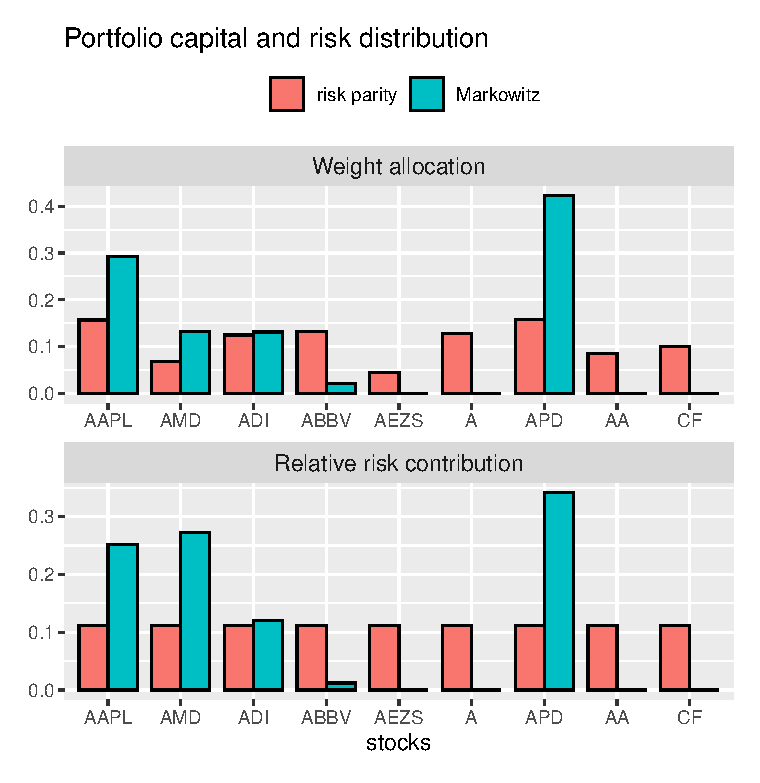
\includegraphics[scale=.65]{codes/markowitz-rpp-comparison.eps}
                  \end{center}
                \end{frame}

        %\begin{frame}
        %    \frametitle{Problem Formulation}
        %    \vspace{.5cm}
        %    \begin{itemize}
        %      \item volatility:
        %        $\sigma(\bm{w}) = \sqrt{\bm{w}^\top\boldsymbol{\Sigma}\bm{w}}$
        %      \item from Euler's theorem:
        %        \begin{equation*}\sigma(\bm{w}) = \sum_{i} w_i \dfrac{\partial \sigma(\bm{w})}{\partial w_i}
        %        = \sum_{i} \dfrac{w_i \left(\boldsymbol{\Sigma}\bm{w}\right)_{i}}{\sqrt{\bm{w}^\top\boldsymbol{\Sigma}\bm{w}}} \end{equation*}
        %      \item $\dfrac{\partial \sigma(\bm{w})}{\partial w_i}$: \textbf{marginal risk contribution}
        %      \item measures the sensitivity of the portfolio volatility to the $i$-th asset
        %      \item it can be defined for other risk measures like VaR and CVaR
        %    \end{itemize}
        %\end{frame}

        %\begin{frame}
        %  \frametitle{Problem Formulation}
        %  \vspace{.75cm}
        %  \begin{itemize}
        %    \item \textbf{risk contribution} of the $i$-th asset to the total risk $\sigma(\bm{w})$:
        %      \begin{equation*}
        %        \textsf{RC}_{i} = w_i \dfrac{\partial \sigma(\bm{w})}{\partial w_i}
        %      \end{equation*}
        %    \item from Euler's theorem:
        %      \begin{equation*}
        %        \sum_{i}\textsf{RC}_i = \sigma(\bm{w})
        %      \end{equation*}
        %    \item \textbf{relative risk contribution} of the $i$-th asset to the total risk $\sigma(\bm{w})$:
        %      \begin{equation*}
        %        \textsf{RCC}_i = \dfrac{\textsf{RC}_i}{\sigma(\bm{w})} = \dfrac{w_i\left(\boldsymbol{\Sigma\bm{w}}\right)_i}{\bm{w}^\top\boldsymbol{\Sigma}\bm{w}},
        %      \end{equation*}
        %      so that
        %      \begin{equation*}
        %        \sum_{i}\textsf{RCC}_i = 1
        %      \end{equation*}
        %  \end{itemize}
        %\end{frame}

        \begin{frame}
          \frametitle{Risk Parity: Problem Formulation}
          \vspace{.5cm}
            \begin{itemize}
              \item \textbf{risk parity portfolio}: $\textsf{RCC}_i = b_i,~i=1,2,\dots,N$
              \item \textbf{feasibility} problem:
            \begin{equation*}
            \begin{array}{ll}
              \underset{\bm{w} \succ \mathbf{0}}{\textsf{find}} & \bm{w} \\
              \textsf{subject to} &
              \dfrac{w_i\left(\boldsymbol{\Sigma\bm{w}}\right)_i}{\bm{w}^\top\boldsymbol{\Sigma}\bm{w}} =
              b_i,~ i = 1, 2, \dots, N
            \end{array}
            \end{equation*}
            doesn't look trivial
          \item \textbf{approximation}: $\boldsymbol{\Sigma}$ is diagonal
            \begin{equation*}
              w_i \propto \dfrac{\sqrt{b_i}}{\sqrt{\boldsymbol{\Sigma}_{ii}}}
            \end{equation*}
          i.e. \textbf{inverse volatility portfolio}
            \end{itemize}
        \end{frame}

        \begin{frame}
          \frametitle{Solution to Risk Parity}
          \vspace{.5cm}
          \begin{itemize}
            \item Spinu (2013):
            \begin{itemize}
            \item change of variables $\bm{x} = \dfrac{\bm{w}}{\sqrt{\bm{w}^\top\boldsymbol{\Sigma}\bm{w}}}$, then $\bm{w} = \dfrac{\bm{x}}{\mathbf{1}^\top\bm{x}}$
            \item problem becomes: $\boldsymbol{\Sigma}\bm{x} = \dfrac{\bm{b}}{\bm{x}}$
            \item $\underset{\bm{x} \succ \mathbf{0}}{\textsf{minimize}} ~f(\bm{x}) = \dfrac{1}{2}\bm{x}^\top\boldsymbol{\Sigma}\bm{x} - \bm{b}^\top\log(\bm{x})$
            \item \textbf{optimality condition:} $\nabla f(\bm{x}) = \boldsymbol{\Sigma}\bm{x} - \dfrac{\bm{b}}{\bm{x}} = \mathbf{0}$
            \item then done? it's not a QP, LP, etc.
           \end{itemize}
          \end{itemize}
        \end{frame}

        \begin{frame}{Cyclical Coordinate Descent (CCD)}
          \vspace{.5cm}
          Griveau-Billion (2013):

          \begin{algorithm}[H]
            \SetAlgoLined
            \caption{CCD to solve risk parity}
            $k \leftarrow 0$, initial $\bm{x}^{(0)}$\\
            \While{not converged}{
              \For{$i = 1$ to $N$}{
                $x_i^{k+1} \leftarrow \underset{x_i}{\textsf{arg min}} f\left(x_{1}^{k+1}, \dots, x_{i}^{k},
                \dots, x_{N}^{k}\right)$
              }
            }
          \end{algorithm}
          \begin{itemize}
            \item closed-form update:
          \end{itemize}
          \begin{equation*}
            x_i^\star = \frac{-\left(\bm{x}_{-i}^\top\boldsymbol{\Sigma}_{:,i}\right)+\sqrt{\left(\bm{x}_{-i}^\top\boldsymbol{\Sigma}_{:,i}\right)^2+
            4\boldsymbol{\Sigma}_{ii}b_i}}{2\boldsymbol{\Sigma}_{ii}},
          \end{equation*}
          where $\bm{x}_{-i} = \left[x_1, \dots, x_{i-1}, 0, x_{i+1}, \dots, x_{N}\right]^\top$
        \end{frame}

        \begin{frame}{Non-convex Formulations}
          \vspace{.5cm}
          \begin{itemize}
            \item limitations of the previous formulation: $\bm{w} \succ \mathbf{0}$, $\mathbf{1}^\top\bm{w} = 1$
            \pause
            \vspace{.25cm}
            \item in practice we would like to include $\bm{l} \preceq \bm{w} \preceq \bm{u}$, $\bm{w}^\top\boldsymbol{\mu}$
            \pause
            \vspace{.25cm}
            \item Bruder \& Roncalli (2012):
              \begin{equation*}
              \begin{array}{ll}
                \underset{\bm{w}}{\textsf{minimize}} &
                \sum_{i=1}^{N}\left(\dfrac{w_i(\boldsymbol{\Sigma}\bm{w})_i}{\bm{w}^\top\boldsymbol{\Sigma}\bm{w}} - b_i\right)^2\\
                \textsf{subject to} & \mathbf{1}^\top\bm{w} = 1, ~\bm{w} \in \mathcal{W}
              \end{array}
              \end{equation*}
            \vspace{.25cm}
            \pause
            \item how to "solve" the non-convex formulation?
            \vspace{.25cm}
            \pause
            \item general purpose solvers: slow \Sadey
            \end{itemize}
        \end{frame}

        \begin{frame}{Non-convex Formulations}
            \vspace{.5cm}
          \begin{itemize}
            \item Feng \& Palomar (2015):
              \begin{equation*}
              \begin{array}{ll}
                \underset{\bm{w}}{\textsf{minimize}} &
                \sum_{i=1}^{N}\left[g_{i}(\bm{w})\right]^2 + \lambda F(\bm{w})\\
                \textsf{subject to} & \mathbf{1}^\top\bm{w} = 1, ~\bm{w} \in \mathcal{W}
              \end{array}
              \end{equation*}
            \end{itemize}
            \begin{itemize}
            \pause
            \item "convexify" the objective function: fast \Laughey
            \vspace{.25cm}
            \pause
            \item \textbf{basic idea}: find a "nice" approximation to the non-convex term, solve it, repeat (Scutari et al. 2014)
            \vspace{.25cm}
            \pause
            \item "nice" approximation for $g_i(\bm{w})$: first order Taylor expansion (Feng \& Palomar 2015)
          \end{itemize}
        \end{frame}

        \begin{frame}{Open Source Software Packages}
          \begin{itemize}
            \item[] \includegraphics[scale=.1]{images/github.png}  dppalomar/riskParityPortfolio (R version)
            \item[] \includegraphics[scale=.1]{images/github.png} dppalomar/riskparity.py (Python version)
          \end{itemize}
          \begin{figure}[!htb]
            \centering
            \includegraphics[scale=0.1]{images/r.png}~
            \includegraphics[scale=0.2]{images/python.png}
          \end{figure}
        \end{frame}

        \begin{frame}[fragile]
          \frametitle{Basic Usage}
          \vspace{.5cm}
          \begin{itemize}
            \item \texttt{R} version:
          \end{itemize}
            \pause
\begin{minted}[
  frame=lines,
  framesep=2mm,
  baselinestretch=1.2,
  fontsize=\footnotesize,
  ]{R}
> library(riskParityPortfolio)
> my_portfolio <- riskParityPortfolio(Sigma = Sigma, b = b)
> names(my_portfolio)
[1] "w"                 "risk_contributions"
\end{minted}
            \pause
          \begin{itemize}
            \item \texttt{Python} version:
          \end{itemize}
\begin{minted}[
  frame=lines,
  framesep=2mm,
  baselinestretch=1.2,
  fontsize=\footnotesize,
  ]{python}
>>> import riskparityportfolio as rp
>>> my_portfolio = rp.RiskParityPortfolio(covariance=Sigma,
                                          budget=b)
>>> my_portfolio.design()
>>> my_portfolio.weights.numpy()
>>> my_portfolio.risk_contributions.numpy()
\end{minted}
        \end{frame}

\begin{frame}[fragile]
\frametitle{Practical Example}
\vspace{.7cm}
\begin{minted}[
  framesep=2mm,
  baselinestretch=1.2,
  fontsize=\footnotesize,
  ]{R}
library(portfolioBacktest)
library(riskParityPortfolio)
# download price data
faang_data <- stockDataDownload(
                  c("GOOG", "NFLX", "AAPL", "AMZN", "FB"),
                   from = "2014-01-01", to = "2019-06-25")
risk_parity <- function(dataset) {
  prices <- dataset$adjusted
  log_returns <- diff(log(prices))[-1]
  return(riskParityPortfolio(cov(log_returns))$w)
}
bt <- portfolioBacktest(
        list("risk parity" = risk_parity,
             "tangency"    = max_sharpe_ratio),
        list(faang_data), T_rolling_window = 12*20,
        optimize_every = 3*20, rebalance_every = 3*20)
\end{minted}
\end{frame}


\begin{frame}[fragile]
  \frametitle{Practical Example}
\begin{minted}[
framesep=2mm,
baselinestretch=1.2,
fontsize=\footnotesize,]{R}

backtestChartStackedBar(bt, portfolio = "tangency",
                        legend = TRUE)
\end{minted}
\begin{figure}[!htb]
  \centering
  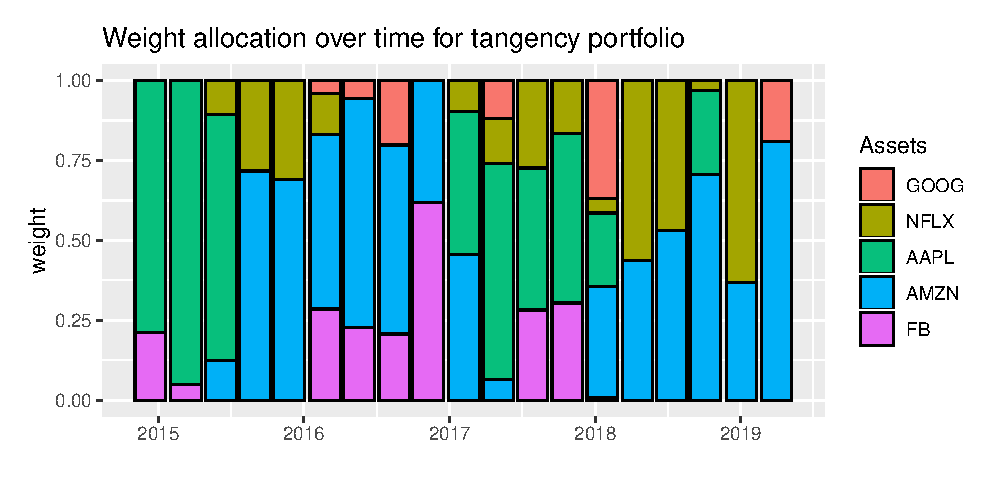
\includegraphics[scale=.7]{codes/weights-msr.eps}
\end{figure}
\end{frame}


\begin{frame}[fragile]
  \frametitle{Practical Example}
\begin{minted}[
framesep=2mm,
baselinestretch=1.2,
fontsize=\footnotesize,]{R}

backtestChartStackedBar(bt, portfolio = "risk parity",
                        legend = TRUE)
\end{minted}
\begin{figure}[!htb]
  \centering
  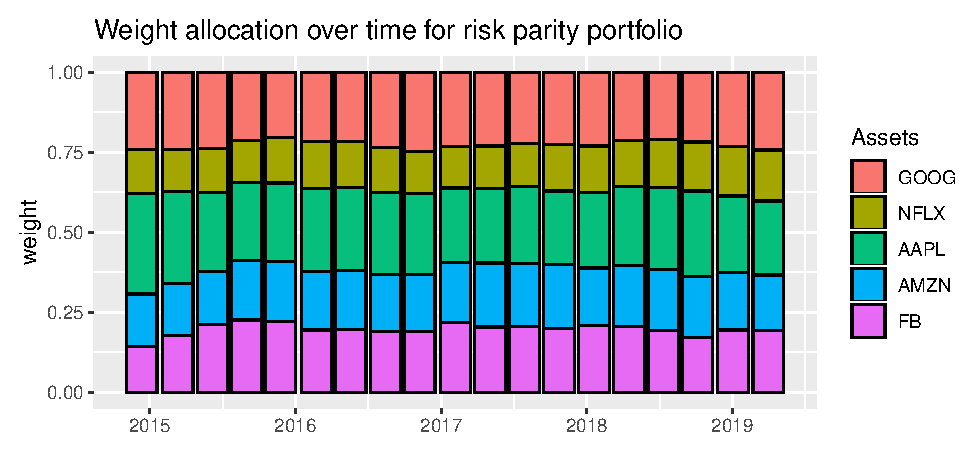
\includegraphics[scale=.7]{codes/weights-rpp.eps}
\end{figure}
\end{frame}


\begin{frame}[fragile]
\frametitle{Practical Example}
\begin{minted}[
  framesep=2mm,
  baselinestretch=1.2,
  fontsize=\footnotesize,
]{R}
backtestChartCumReturns(bt) + theme(legend.position="top")
\end{minted}
\begin{figure}[!htb]
  \centering
  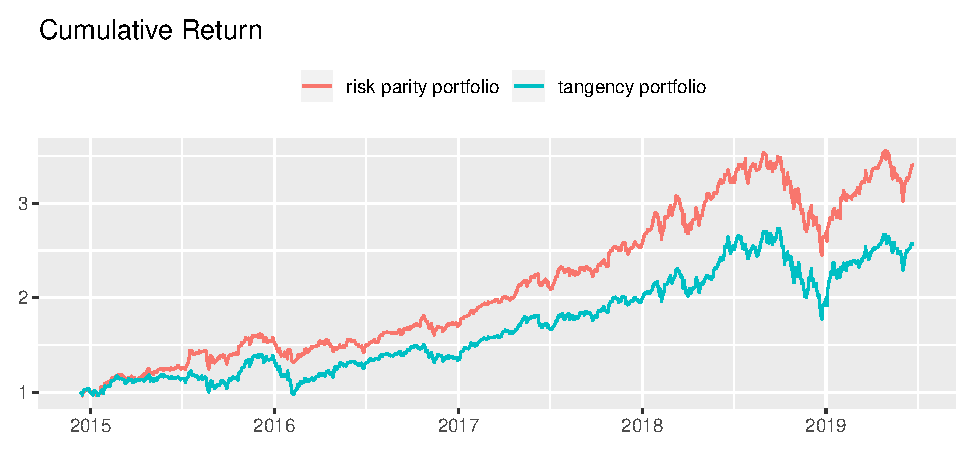
\includegraphics[scale=.7]{codes/returns.eps}
\end{figure}
\end{frame}

\begin{frame}{Testimonials}
  \vspace{.5cm}
  "I can easily run optimizations across new covariance matrices in seconds, which has helped streamline portfolio allocation testing"\linebreak
  \begin{flushright}Jonathan Dane, CFA. Director of Portfolio Strategy \& Market Research, The Coury Firm.\end{flushright}

    "\textbf{riskParityPortfolio} provides a state-of-the-art
   implementation of rpps, otherwise only available at the top quantitative
   hedge funds"\linebreak
   \begin{flushright}Tharsis Souza, PhD. Director of Strategic Innovation, Axioma Inc. Founder, OpenQuants.com.\end{flushright}

   {\footnotesize Disclaimer: views, thoughts, and opinions expressed in the text belong solely to the author,
   and not necessarily to the author’s employer, organization, committee or other group or individual.}
\end{frame}


\begin{frame}{Takeaways}
  \vspace{.5cm}
  \begin{enumerate}
    \item risk parity represents a shift from \textbf{capital} allocation to \textbf{risk} allocation
            \pause
        \vspace{.25cm}
    \item risk parity portfolios have been praised for their robustness in different market "weathers"
            \pause
        \vspace{.25cm}
    \item non-convex? no problem!
            \pause
        \vspace{.25cm}
    \item GitHub repositories to stay tuned:
      \begin{itemize}
        \item dppalomar/riskParityPortfolio
        \item dppalomar/riskparity.py
        \item dppalomar/portfolioBacktest
      \end{itemize}
  \end{enumerate}
\end{frame}

\section{Thank you! Questions?}

\begin{frame}{References}
  \vspace{.5cm}
  \begin{itemize}
    \item {\footnotesize H .M. Markowitz. "Portfolio selection". The Journal of Finance. 7 (1): 77–91, 1952.}
    \item {\footnotesize Y. Feng and D. Palomar, "SCRIP: Successive convex optimization methods for risk parity portfolios design,"
           IEEE Trans. Signal Process., vol. 63, no. 19, pp. 5285–5300, 2015.}
    \item {\footnotesize Scutari et al. "Decomposition by partial linearization: Parallel optimization of multi-agent systems".
           IEEE Trans. Signal Processing, 62(3), 641–656, 2014.}
    \item {\footnotesize B. Bruder and T. Roncalli, "Managing risk exposures using the risk budgeting approach".
           University Library of M\"unich, Germany, Tech. Rep., 2012.}
    \item {\footnotesize F. Spinu, "An algorithm for computing risk parity weights". SSRN, 2013.}
    \item {\footnotesize T. Griveau-Billion, "A fast algorithm for computing high-dimensional risk parity portfolios".
           \url{https://www.thierry-roncalli.com/download/CCD-Risk-Parity.pdf}, 2013.}
    \item {\footnotesize T. Souza, "DIY Ray Dalio ETF: How to build your own Hedge Fund strategy with risk parity portfolios".
           \url{https://www.openquants.com}}
  \end{itemize}
\end{frame}
\end{document}
